\documentclass{beamer}

\usepackage{graphicx}
\usepackage{verbatim}
\usepackage[mediumspace,mediumqspace,squaren,binary]{SIunits}


%\includeonlyframes{1,2,3}

\usetheme{Antibes}
\usecolortheme[RGB={32,115,53}]{structure} %green

\usebackgroundtemplate{
  % UniCT Logo
  
\includegraphics[width=370pt]{img/unict.jpg}
}

%%\newtheorem{samplecode}{Sample Code}

%\setbeamercovered{transparent}
\setbeamertemplate{blocks}[rounded][bg=red]
\setbeamertemplate{footline}[frame number]{}


\newcommand{\bigtilde}{$\sim$}

% Spaces
\newcommand{\N}{\vskip 0.3 cm}
\newcommand{\n}{\vskip 0.2 cm}
\newcommand{\TAB}{\hskip 1.8 cm}
\newcommand{\tab}{\hskip 0.6 cm}

% Colors
\newcommand{\red}[1]{\textcolor[rgb]{.8,0,0}{#1}}
\newcommand{\blue}[1]{\textcolor[rgb]{0,0,.7}{#1}}
\newcommand{\navy}[1]{\textcolor[rgb]{0,0,.5}{#1}}
\newcommand{\purple}[1]{\textcolor[rgb]{.7,0,.8}{#1}}
\newcommand{\green}[1]{\textcolor[rgb]{0,.6,.1}{#1}}


\title[Un sistema per il monitoraggio di impianti fotovoltaici]{
  Un sistema per il monitoraggio di \\ impianti fotovoltaici
 }\subtitle[]{Progetto e implementazione}
\author{Loris Fichera \n
Relatore: Prof. Corrado Santoro}
\institute[Universit\`a di Catania]{
	Universit\`a degli Studi di Catania\\
        Corso di Laurea Specialistica in Ingegneria Informatica\\
}
\date{20 Luglio 2011}

\begin{document}

% Title Page
\begin{frame}[plain]
  \titlepage
\end{frame}
%

%% \begin{frame}
%% \tableofcontents
%% \end{frame}

%% \section{Introduzione}
%% \begin{frame}{Monitoraggi \emph{immaturi}}
%%   Il numeri del fotovoltaico in Italia (\red{GSE}):
%%   \begin{itemize}
%%   \item oltre \red{4 GWp} al 31/12/2010
%%   \item potenza installata \red{raddoppia} ogni anno
%%   \end{itemize}
%%   \N
%%   Monitorare gli impianti fotovoltaici diventa importante per
%%     \begin{itemize}
%%     \item i \green{soggetti responsabili}
%%     \item gli \green{installatori/manutentori}
%%   \end{itemize}
%%   \N  
%%   "Gran parte delle soluzioni oggi in commercio mostrano caratteri di \emph{immaturit\`a}" (C. Podewils 2010)
%% \end{frame}
%

%
\section{Il monitoraggio degli impianti fotovoltaici}
\subsection{Definizione del Problema}
\begin{frame}{Obiettivi}
  Un sistema di monitoraggio effettua la \green{raccolta} e \green{l'integrazione} dei  \red{dati rilevanti} di un impianto al fine di
  determinarne:
%
\begin{itemize}
\item lo stato operativo
\item l'efficienza globale
\item la produzione energetica
\end{itemize}
%
\begin{figure}[!h]
  \begin{center}
    \fbox{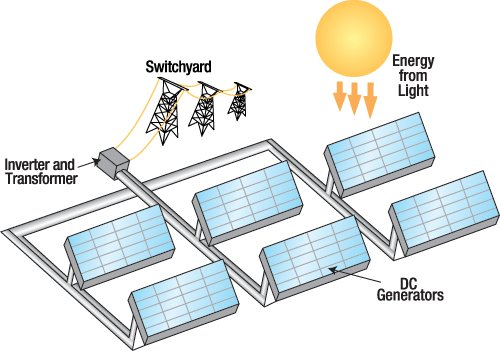
\includegraphics[width=140pt]{img/solar_photovoltaic.jpg}}
  \end{center}
\end{figure}
%
Quali sono i \red{dati rilevanti}?
\end{frame}
%

%
\begin{frame}{Classi di utenti (Kolodenny 2008)}
Kolodenny \emph{et al.}, identificano le seguenti \green{classi di utenti}:
\N
%
\begin{itemize}
%% \item \red{ricercatore}
%%   \begin{itemize}
%%   \item insieme di grandezze ben definito
%%   %%\item quanti pi\`u dati possibile
%%   \item alto livello di dettaglio
%%   \end{itemize}
  %
\item \red{proprietario}
  \begin{itemize}
  \item energia prodotta
  \item ritorno economico
  \end{itemize}
  %
\item \red{manutentore}
  \begin{itemize}
  \item comportamento di ogni componente (modulo, inverter...)
  \item dati ambientali
  \end{itemize}
\end{itemize}
%
\end{frame}
%

%
\section{La soluzione implementata}
\begin{frame}{Panoramica del sistema}
%
\begin{figure}[!h]
  \begin{center}
    \fbox{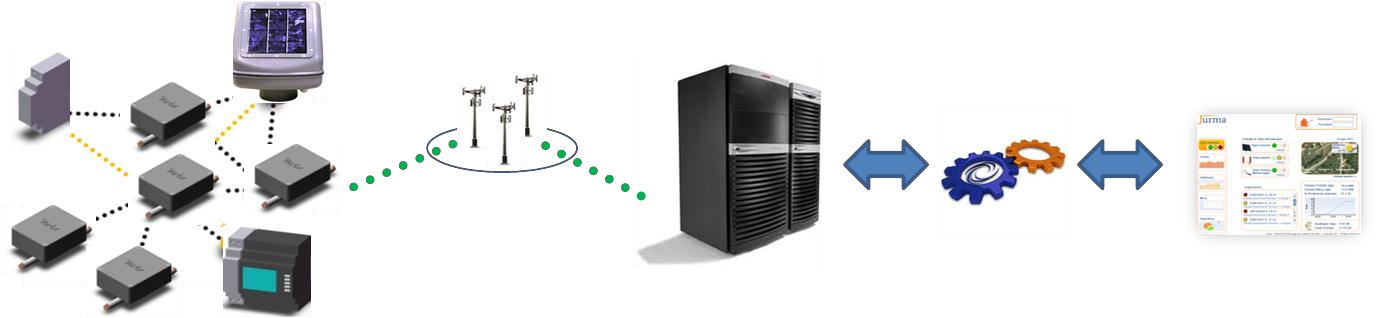
\includegraphics[width=310pt]{img/architecture.png}}
  \end{center}
\end{figure}
%
\begin{itemize}
\item infrastruttura \red{di campo}
\item trasmissione dati via \red{gprs} (o \red{sms})
\item \red{datacenter}
\item accesso ai dati via \red{web services}
\item portale web
\end{itemize}
%
\end{frame}
%

%
\subsection{L'infrastruttura di campo}
\begin{frame}{Infrastruttura di campo}
%
\begin{itemize}
  \item \red{Wireless Sensor Network} (WSN) ZigBee-based
    \begin{itemize}
    \item bassi costi
    \item facilit\`a di installazione
      \begin{itemize}
      \item no cablaggi aggiuntivi
      \item rete autoconfigurante
      \end{itemize}
    \end{itemize}
    \N
  \item previsti tre tipi di nodi
    \begin{itemize}
    \item \red{gateway}
    \item \red{power/inverter transponder}
    \item \red{string transponder}
    \end{itemize}
\end{itemize}
%
\end{frame}
%

%
\begin{frame}{Nodi WSN}
    \begin{columns}
      \column{1.7in}
  \begin{figure}[!h]
    \begin{center}
      \fbox{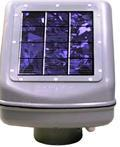
\includegraphics[width=50pt]{img/gw.jpg}}\\
      \fbox{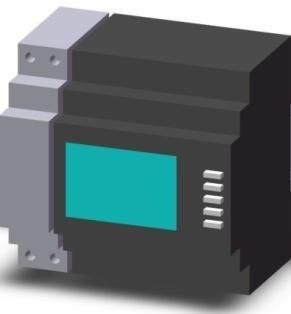
\includegraphics[width=50pt]{img/power-transponder.jpg}}\\
      \fbox{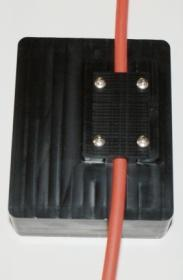
\includegraphics[width=40pt]{img/string-transponder.jpg}}
    \end{center}
  \end{figure}
      \column{2.5in}
      \begin{itemize}
      \item \red{Gateway}
        \begin{itemize}
        \item concentratore dati
        \item trasmette dati via \green{gprs}/\green{sms}
        \item effettua misure di irraggiamento
        \end{itemize}
        \N \N

      \item \red{Power/Inverter Transponder}
        \begin{itemize}
        \item misura di \green{grandezze elettriche}\\
          (corrente, tensione, PF...)
        \end{itemize}
        \N \N

      \item \red{String Transponder}
        \begin{itemize}
        \item misura della \green{corrente di stringa}
        \item sensore a \green{effetto Hall}
        \end{itemize}

      \end{itemize}
    \end{columns}
\end{frame}


%% \begin{frame}{Il Gateway}
%%   \begin{figure}[!h]
%%   \begin{center}
%%     \fbox{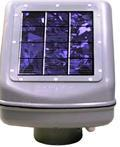
\includegraphics[width=60pt]{img/gw.jpg}}
%%   \end{center}
%% \end{figure}
%% %
%% \begin{itemize}
%%   \item agisce da \red{concentratore dati}
%%   \item \red{modem gsm} per la trasmissione dei dati
%%     \begin{itemize}
%%     \item via \green{sms}
%%     \item via \green{FTP} \emph{over} \green{gprs}
%%     %%\item \red{transmission interval} configurabile
%%       \end{itemize}
%%   \item \red{elemento fotovoltaico} per la ricarica della batteria
%% \end{itemize}
%% %
%% \end{frame}
%% %

%% %
%% \begin{frame}{Il Power/Inverter Transponder}
%% \begin{figure}[!h]
%%   \begin{center}
%%     \fbox{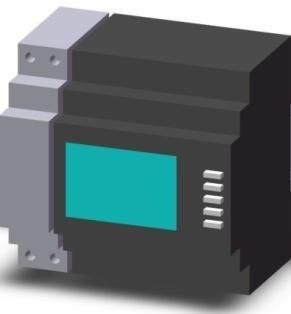
\includegraphics[width=60pt]{img/power-transponder.jpg}}
%%   \end{center}
%% \end{figure}
%% %
%% \begin{itemize}
%% \item \red{analizzatore di rete} + \red{transponder ZigBee}
%% \item misura delle grandezze elettriche \\ (corrente, potenza, power factor...)
%%   \begin{itemize}
%%   \item a monte del contatore bidirezionale
%%   \item a valle di ogni inverter
%%   \item \red{sampling interval} configurabile
%%   \end{itemize}
%% \end{itemize}
%% %
%% \end{frame}
%% %

%% %
%% \begin{frame}{Lo String Transponder}
%% \begin{figure}[!h]
%%   \begin{center}
%%     \fbox{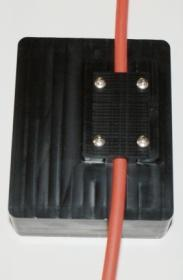
\includegraphics[width=60pt]{img/string-transponder.jpg}}
%%   \end{center}
%% \end{figure}
%% %
%% \begin{itemize}
%% \item \red{sensore di corrente} (a \emph{effetto Hall}) + \red{transponder ZigBee}
%% \item misura della corrente di stringa
%%   \begin{itemize}
%%   \item \red{sampling interval} configurabile  
%%   \end{itemize}
%%   \end{itemize}
%% \end{frame}
%

%
\subsection{Il Datacenter}
%
\begin{frame}{Il Datacenter}
Si occupa di
\begin{itemize}
\item \green{gestire i flussi informativi} generati dai gateway
\item \green{elaborare} e \green{memorizzare} i dati di campo 
\item generare \green{report} e \green{allarmi}
\item fornire \green{accesso ai dati} mediante \green{web services RESTful}
\end{itemize}
%
\N
\begin{itemize}
  \item \`e interamente basato su \red{Erlang/OTP}
  \item \`e costituito da un insieme di \red{Erlang applications}
\end{itemize}
%
\begin{figure}[!h]
  \begin{center}
    \fbox{
\includegraphics[width=60pt]{img/erlang-logo.png}}
  \end{center}
\end{figure}
%
\end{frame}
%

%
%% \begin{frame}[fragile]{L'applicazione \texttt{database}}
%%   Possiede un unico processo \green{worker}, il quale 
%%   funge da wrapper per il database \red{MySQL} in cui vengono memorizzati
%%   \begin{itemize}
%%   \item configurazioni degli impianti
%%   \item dati di monitoraggio
%%   \end{itemize}
%%   %
%% \begin{exampleblock}{Code snippet}
%% \begin{semiverbatim}
%% data_storage:\red{add_new_plant_by_structure} (
%%       \green{_UniqueID} = "MyPlant", 
%%       \green{_Location} = "Nowhere",
%%       ...
%%       \green{_Inverters} = [{{"YURAKU", "I-3000"}, 
%%                     "Inverter-00", "0000-0000-0000", 
%%                     [%% strings here...
%%                      ]} ]).
%% \end{semiverbatim}
%% \end{exampleblock}  
%% \end{frame}
%

%
%% \begin{frame}{L'applicazione \texttt{sysconf}}
%% \end{frame}
%

%
\begin{frame}{L'applicazione \texttt{datamanager}}
%
Gestisce i flussi informativi generati da ogni impianto
%
\begin{figure}[!h]
  \begin{center}
    \fbox{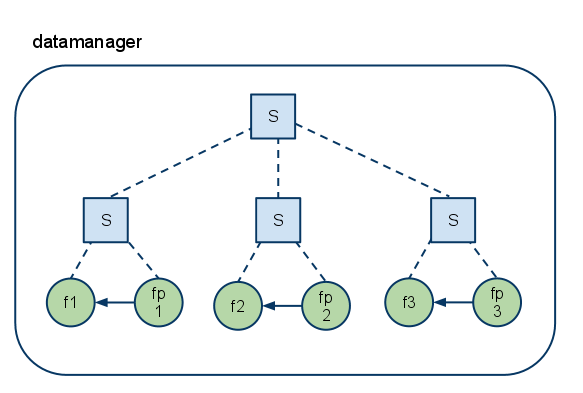
\includegraphics[width=150pt]{img/datamanager.png}}
  \end{center}
\end{figure}
%
\begin{itemize}
\item un \emph{process pool} per ogni impianto
\item due \red{worker} per \emph{pool}
  \begin{itemize}
  \item un \texttt{filter}
  \item un processo \red{endpoint} (\texttt{file\_poller}, \texttt{sms\_manager})
  \end{itemize}
%%\item politiche di \red{riavvio} dei supervisor
\end{itemize}
%
\end{frame}
%

%
\begin{frame}[fragile]{Il \texttt{file\_poller}}
  %
  \begin{itemize}
  \item decodifica i dati ricevuti via \red{FTP}
  \item genera \red{report} riguardo
    \begin{itemize}
    \item dati \red{corrotti}
    \item dati \red{mancanti}
    \end{itemize}
  \item invia i dati ricevuti al \texttt{filter}
  \end{itemize}
  %
\begin{exampleblock}{Decodifica dei dati}
\begin{semiverbatim}
\begin{small}
\green{try}
 \{ok, \blue{FileContent}\} = 
   \red{file:read_file} (lists:concat ([Path, File])),
   \red{ftp_protocol:decode} (\blue{FileContent})
		
\green{catch} error : \{\blue{Reason}, D\} ->
    ...
  nil
\green{end},
\end{small}
\end{semiverbatim}
\end{exampleblock}  
\end{frame}
%

%
\begin{frame}{Il \texttt{filter}/1}
%
Due attivit\`a concorrenti:
\begin{itemize}
\item \red{filtraggio} dei dati ricevuti (scaling, ecc.)
\item \red{stima} di altri valori
\end{itemize}  
%
\begin{figure}[!h]
  \begin{center}
    \fbox{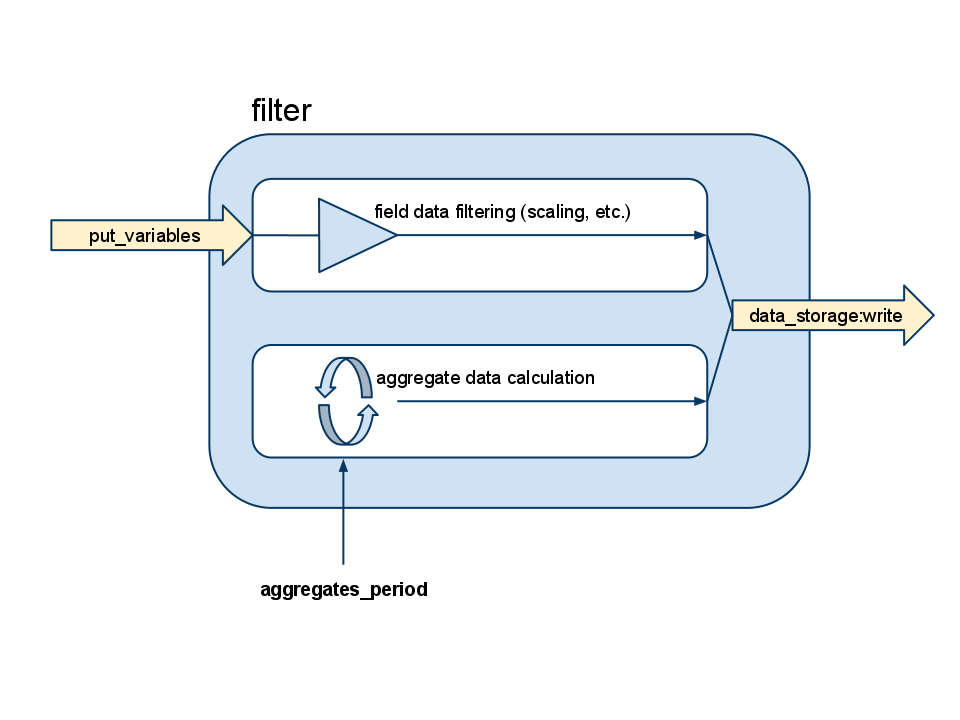
\includegraphics[width=190pt]{img/filter.png}}
  \end{center}
\end{figure}
\end{frame}
%

%
\begin{frame}[fragile]{Il \texttt{filter}/2}
  \begin{exampleblock}{Calcolo della potenza totale per Power Transponder}
    \begin{semiverbatim}
      \begin{small}
\{ok, \{_, \blue{Vars}\}\} = 
  \red{data_storage:get_trend_by_device} (\blue{DeviceID}, F, T, 
                                   ["active-power-l1",
                                    "active-power-l2",
                                    "active-power-l3"]),
	      
\blue{PropList} = \red{measure_data_to_proplist} (\blue{Vars}),
\blue{P1} = \red{proplists:get_value} ("active-power-l1", \blue{PropList}),
\blue{P2} = \red{proplists:get_value} ("active-power-l2", \blue{PropList}),
\blue{P3} = \red{proplists:get_value} ("active-power-l3", \blue{PropList}),
	      
\blue{TotalActivePower} = \blue{P1} + \blue{P2} + \blue{P3}, 
\end{small}
    \end{semiverbatim}
  \end{exampleblock}
\end{frame}


%% \begin{frame}[fragile]{Web Services}
%%   \begin{itemize}
%%   \item basati su \red{Yaws}
%%   \item \red{RESTful}
%%   \end{itemize}
%% %
%%   \begin{exampleblock}{Servizio \texttt{get\_plants}}
%%     \begin{semiverbatim}
%%       \begin{small}
%% <erl>
%% out(A) ->
%%  \{ok, \blue{PlantList}\} = \red{data_storage:get_plants}(),
%%   Reply =
%%     \red{xml_translator:make_plant_list_response} (\blue{PlantList}),
%%   {html, \blue{Reply}}.
%% </erl>

%% <\purple{plant_list_response}>
%%   <\purple{plant} \navy{id}="1" \navy{unique_id}="plant-1" \navy{customer_id}="0" ... />
%% </\purple{plant_list_response}>
%%       \end{small}
%%     \end{semiverbatim}
%%   \end{exampleblock}
%% \end{frame}

\section{Testing}
%% \begin{frame}{Corrente immessa in rete vs. Potenza prodotta}
%%   \begin{columns}
%%     \column{2.5in}
%%     \begin{figure}[!h]
%%       \begin{center}
%%         \fbox{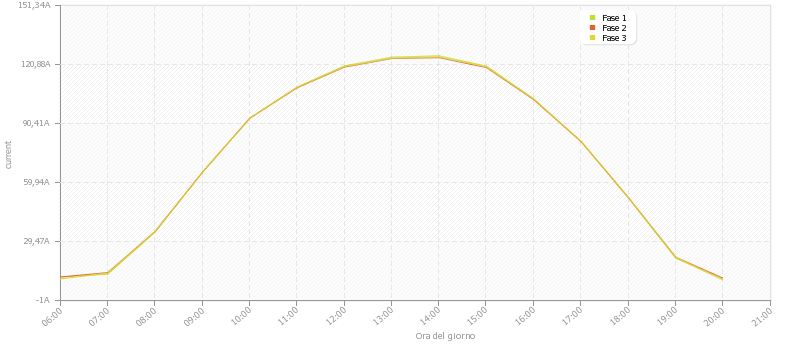
\includegraphics[width=145pt]{img/current-power-transponder.png}}
%%       \end{center}
%%     \end{figure}
%%     %   
%%     \begin{figure}[!h]
%%       \begin{center}
%%         \fbox{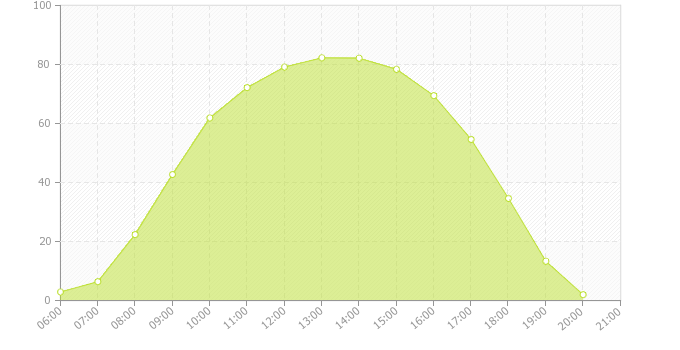
\includegraphics[width=145pt]{img/potenza-giornaliera.png}}
%%       \end{center}
%%     \end{figure}
%%     %
%%     \column{1.7in}
%%     %
%%     \textbf{Configurazione}
%%     \begin{itemize}
%%     \item \textbf{1} Power Transponder
%%     \item \textbf{1} Gateway
%%     \end{itemize}
%%     %
%%     \N
%%     %
%% %%    \textbf{Valori di picco} (14\:00hrs)
%%     \textbf{Valori di picco} (1400hrs)
%%     \begin{itemize}
%%     \item \textbf{\bigtilde{} 120 \ampere} per fase
%%     \item \textbf{\bigtilde{} 82 \kilo\watt}
%%     \end{itemize}
    
%%   \end{columns}
%% \end{frame}
%

%
\begin{frame}{Radiazione vs. Potenza prodotta}
  \begin{columns}
    \column{2.5in}
    \begin{figure}[!h]
      \begin{center}
        \fbox{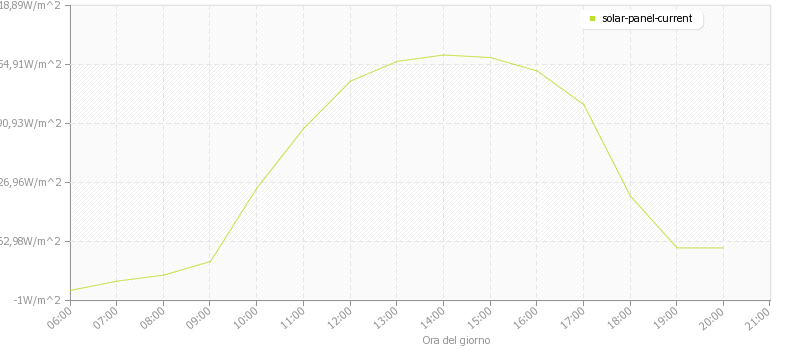
\includegraphics[width=150pt]{img/radiazione-giornaliera.png}}
      \end{center}
    \end{figure}
    %   
    \begin{figure}[!h]
      \begin{center}
        \fbox{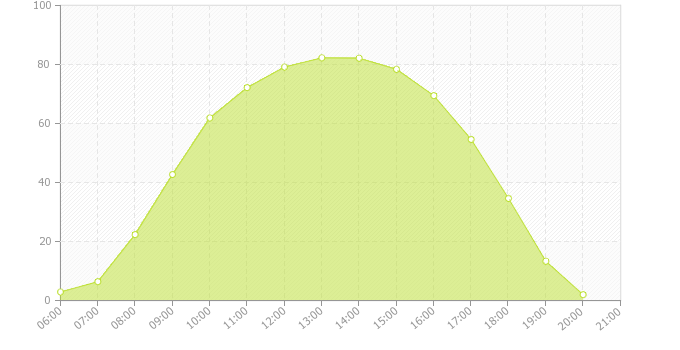
\includegraphics[width=145pt]{img/potenza-giornaliera.png}}
      \end{center}
    \end{figure}
    \column{1.7in}
    %
    \textbf{Configurazione}
    \begin{itemize}
    \item \textbf{1} Power Transponder
    \item \textbf{1} Gateway
    \end{itemize}
    %
    \N
    %
%%    \textbf{Valori di picco} (14\:00hrs)
    \textbf{Valori di picco} (1400hrs)
    \begin{itemize}
    \item \textbf{\bigtilde{} 900 \watt\per\squaremetre}
    \item \textbf{\bigtilde{} 82 \kilo\watt}
    \end{itemize}

    \end{columns}
\end{frame}
%

%
\section{Sviluppi futuri}
%
\begin{frame}{Sviluppi futuri}
  \begin{itemize}
    \item \red{sicurezza} delle comunicazioni Gateway - Datacenter
    \item \red{sistema esperto} per la diagnosi delle anomalie
  \end{itemize}
   \begin{figure}[!h]
      \begin{center}
        \fbox{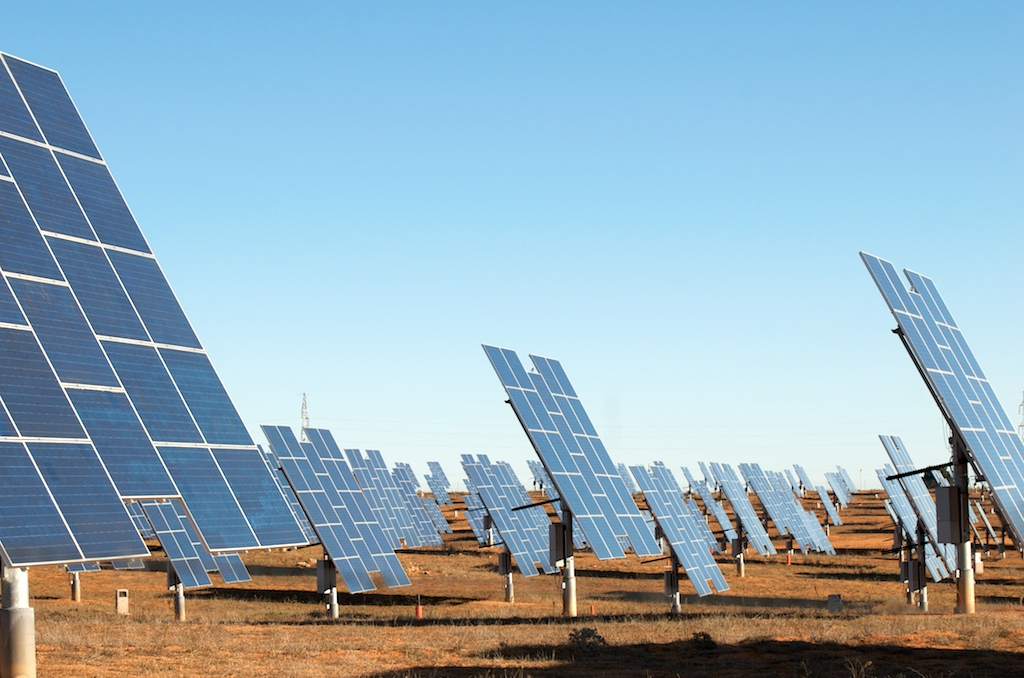
\includegraphics[width=200pt]{img/solar-plant.jpg}}
      \end{center}
    \end{figure}
\end{frame}
%
\end{document}
